
\chapter{Evaluation des Beschneidens des Netzes}\label{sec:ptexperimente}
\section{Evaluation bei gleichbleibender Batchgröße}

Die Untersuchung von PruneTrain basiert auf einer bereits vorgefertigten Implementierung \cite{ptImpl}. In dieser Implementierung ist alles bis auf die Anpassung der Batchgröße an das kleiner werdende Netz enthalten. Das Ergebnis der Ausführung von PruneTrain auf der Hardware wird mit den Ergebnissen aus der Veröffentlichung verglichen \cite{prunetrain}. Ziel der Experimente ist es zu evaluieren, wie eine Änderung der verschiedenen Hyperparameter die Trainingszeit und die Accuracy beeinflusst. Im Gegensatz zur Veröffentlichung von PruneTrain wird hier statt auf mehreren GPUs nur auf einer GPU gerechnet. So kann evaluiert werden, wie viel der PruneTrain Effekte auf das Setup mit mehreren GPUs in der Veröffentlichung zurückzuführen sind. 

Bei der Evaluierung der Einflüsse werden die veränderbaren Hyperparameter von PruneTrain einzeln verändert, um den Einfluss der einzelnen Veränderungen zu untersuchen.  
Die veränderbaren Hyperparameter sind\footnote{Diese Größen werden in Kapitel \ref{sec:prunetrain} erklärt}:
\begin{itemize}
 \item Lasso-Ratio $0,2$
 \item Rekonfigurationsinterval $5$
 \item Grenzwert $0,0001$
 \item Lernrate $0,1$
\end{itemize}
Hinter den veränderbaren Hyperparameter steht jeweils der Wert, den der Hyperparameter hat, wenn er im aktuellen Experiment nicht verändert wird.
Betrachte eine feste Batchgröße von 256 über 180 Epochen und vergleiche diese mit dem Baseline-Netzes aus Kapitel \ref{sec:baseline}. Für jede Gruppe von Experimenten werden fünf Experimente durchgeführt. 


\subsubsection{Einfluss von verschiedenen Lasso-Ratio Werten auf das Netz}
Die Lasso-Ratio gibt an, wie stark das Netz beschnitten werden soll. In diesen Experimenten wird die Lasso-Ratio von 0,05 bis 0,25 in 0,05er Schritten verändert. In Abbildung \ref{abb:lasso1} ist zusehen, dass mit steigender Lasso-Ratio durchschnittlich weniger Trainingszeit gebraucht wird. Für die durchschnittliche Trainingszeit eines Experiments wird das arithmetische Mittel über alle Epochen angewandt. Die Experimente werden dann nach ihrer Zugehörigkeit einsortiert und als Boxplot in Abbildung \ref{abb:lasso1} dargestellt. Trotz der nachlassenden Trainingszeit mit steigender Lasso-Ratio ist die Trainingszeit des Baseline-Netzes signifikant schneller. Dies ist durch den Overhead erklärbar, welcher durch das Beschneiden des Netzes entsteht.
Um zu überprüfen, wie signifikante diese Unterschiede zwischen den Experimentengruppen hier sind werden paarweise t-Tests mit einem Signifikanzniveau $\alpha=0,05$ durchgeführt. Die resultierenden p-Werte sind in Tabelle \ref{tab:lasso1} zu sehen.

\begin{table}[]
\centering
\begin{tabular}{l|c|c|c|c|c|}
\cline{2-6}
& \multicolumn{1}{l|}{Lasso $0,05$} & \multicolumn{1}{l|}{Lasso $0,1$} & \multicolumn{1}{l|}{Lasso $0,15$} & \multicolumn{1}{l|}{Lasso $0,2$} & \multicolumn{1}{l|}{Lasso $0,25$} \\ \hline
\multicolumn{1}{|l|}{Baseline}                             & $6,9\cdot10^{-6}$   & $<2,2\cdot10^{-16} $   & $<2,2\cdot 10^{-16}$     & $2,9\cdot 10^{-5}$   & $4,9\cdot10^{-5}$    \\ \hline
\multicolumn{1}{|l|}{Lasso $0,05$}                             & X                               & $0,0299$                         & $0,0199$                          & $0,0002$                         & $5,6\cdot 10^{-5}$    \\ \hline
\multicolumn{1}{|l|}{Lasso $0,1$}                             & X                               & X                              & $0,0025$                          & $0,0035$                         & $0,0016$                          \\ \hline
\multicolumn{1}{|l|}{Lasso $0,15$}   & X                               & X                              & X                               & $0,0046$                         & $0,0019$                          \\ \hline
\multicolumn{1}{|l|}{Lasso $0,2$}                             & X                               & X                              & X                               & X                              & \cellcolor[HTML]{FE0000}$0,2540$                          \\ \hline
\end{tabular}
\caption{p-Werte für den t-Tests zu den durchschnittlichen Trainingszeiten der Lasso-Ratio Experimente}
\label{tab:lasso1}
\end{table}
Da bis auf den t-Test zwischen den Lasso Werten 0,2 und 0,25 alle p-Werte kleiner dem Signifikanzniveau sind ist ein Fehler 1.Art sehr unwahrscheinlich. Daher lässt sich für die übrigen Wertepaare die Aussage treffen, dass sie einen statistisch signifikanten Unterschied der Mittelwerte haben. Somit entsteht durch das Erhöhen der Lasso-Ratio ein signifikante Einsparung an Trainingzeit gegenüber einer kleineren Lasso-Ratio. Gegenüber den durchschnittlichen Trainingszeiten des Baseline-Netzes ist allerdings das Baseline in allen Fällen signifikante schneller.  


In Abbildung \ref{abb:lasso2} ist die Accuracy der verschiedenen Experimente abgebildet. Es fällt auf, dass das Baseline-Netz im Mittel etwas besser ausfällt als die Experimente mit dem Lasso-Ratio 0,05.
\begin{figure}
     \centering
     \subfloat[][]{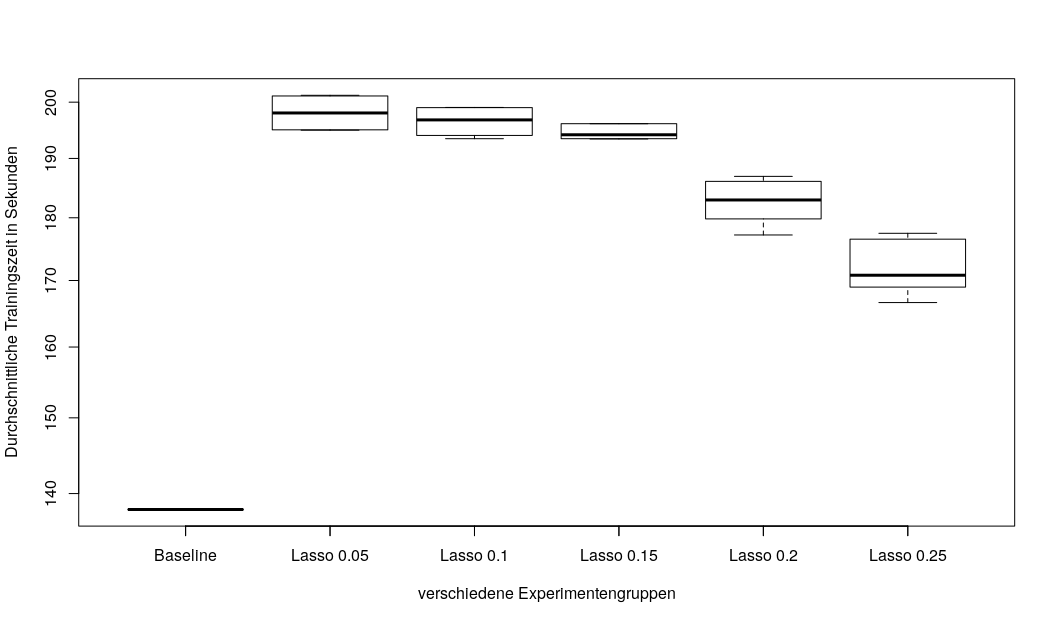
\includegraphics[width= .5\linewidth]{KapitelPartB/Images/lasso1.png}\label{abb:lasso1}}
     \hfill
     \subfloat[][]{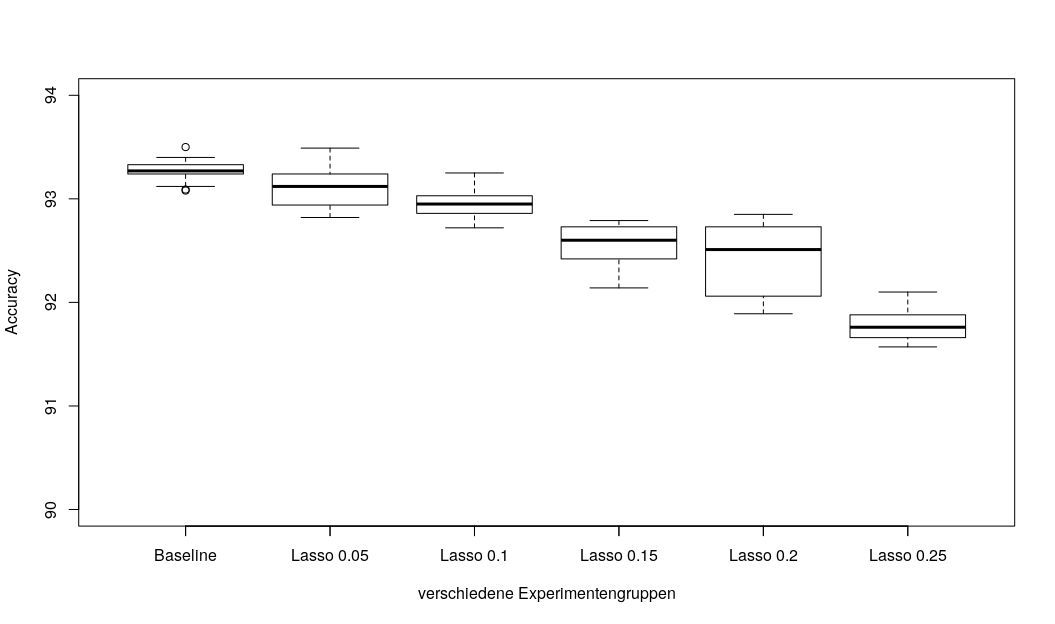
\includegraphics[width=.5\linewidth]{KapitelPartB/Images/lasso2.png}\label{abb:lasso2}}
     \caption{Lasso-Ratio Experiment: (a) Boxplot der durchschnittlichen Trainingszeit (b) Boxplot der Accuracy}
     \label{abb:lasso}
\end{figure}
In Tabelle \ref{tab:lasso2} sind die Werte für den paarweisen t-Test zwischen den Accuracy der Experimentegruppen abgebildet. Das Signifikanzniveau beträgt $\alpha =0,05$. In der Tabelle ist zu sehen, dass die rot hinterlegten p-Werte größer als das Signifikanzniveau sind. Somit ist für diese paarweisen Accuracy die Wahrscheinlichkeit für einen Fehler 1. Art zu groß für die Aussage, dass die Accuracy der Experimente einen unterschiedlichen Mittelwert haben. Es lässt sich jedoch erkennen, dass für jede Zeile die p-Werte kleiner werden, je größer die Lasso-Ratio wird. Somit lässt sich die begründete Aussage treffen, dass mit steigender Lasso-Ratio die Accuracy signifikant abnimmt.
Die fehlende Signifikanz dieser Paare kann sowohl an der fehlenden statistischen Signifikanz liegen als auch an der kleinen Anzahl an Experimenten pro Gruppe. Da die hier getroffene Aussage allerdings ausreicht wird das Experiment nicht mit grösserer Anzahl wiederholt.




\begin{table}[]
\caption{p-Werte für den t-Tests zu den Accuracy-Werten der Lasso-Ratio Experimente}
\centering
\begin{tabular}{l|c|c|c|c|c|}
\cline{2-6}
                                & \multicolumn{1}{l|}{Lasso $0,05$} & \multicolumn{1}{l|}{Lasso $0,1$} & \multicolumn{1}{l|}{Lasso $0,15$} & \multicolumn{1}{l|}{Lasso $0,2$} & \multicolumn{1}{l|}{Lasso $0,25$} \\ \hline
\multicolumn{1}{|l|}{Baseline}   & \cellcolor[HTML]{FE0000}$0,7068$  & \cellcolor[HTML]{FE0000}$0,4952$ & \cellcolor[HTML]{FE0000}$0,2586$  & $0,0018$                         & $8,6\cdot 10^{-6}$     \\ \hline
\multicolumn{1}{|l|}{Lasso $0,05$}& X                               & \cellcolor[HTML]{FE0000}$0,2898$ & \cellcolor[HTML]{FE0000}$0,1341$  & $0,0010$                       & $1,0\cdot 10^{-7}$    \\ \hline
\multicolumn{1}{|l|}{Lasso $0,1$} & X                               & X                              & \cellcolor[HTML]{FE0000}$0,6530$   & $0,0041$         ig              & $7,5\cdot10^{-5}$    \\ \hline
\multicolumn{1}{|l|}{Lasso $0,15$}& X                               & X                              & X                               & $0,0072$                       & $0,0001$                       \\ \hline
\multicolumn{1}{|l|}{Lasso $0,2$} & X                               & X                              & X                               & X                              & $0,0182$                         \\ \hline
\end{tabular}
\label{tab:lasso2}
\end{table}



\subsubsection{Experimente zum Rekonfigurationsintervall}
 Als nächste Größe wird der Einfluss des Rekonfigurationsintervalls überprüft. Die entsprechenden Grafiken sind in Abbildung \ref{abb:reconf} zu sehen. In Abbildung \ref{abb:reconf1} sind für die verschiedenen Experimente die Trainingszeiten pro Epoche zu sehen. Dabei werden drei verschiedene Rekonfigurationsintervalle (2,5 und 10) verglichen. In Abbildung \ref{abb:reconf1} lässt sich für die verschiedenen durchschnittlichen Trainingszeiten der Experimente zum Rekonfigurationsintervall kaum Unterschiede erkennen. Daher ist in Abbildung \ref{abb:reconf2} ein Boxplot ohne die Baseline Werte abgebildet. Der Grund hierfür ist, dass sich die Zeitersparnis durch das vermehrte Beschneiden aufgrund einem kleinerem Rekonfigurationsintervall mit dem nötigen Overhead der häufigeren Rekonfiguration aufhebt.
 
 
 In Tabelle \ref{tab:reconf} ist bestätigt, das zwischen den durchschnittlichen Trainingszeiten der Experimente kein signifikanter Unterschied ist. Dabei ist zu bedenken, dass die Experimentanzahl mit fünf relativ klein ist. Wichtiger als die hier eventuell minimale Einsparung von Trainingszeit ist die Auswirkung auf die Accuracy.
 


\begin{table}[]
\caption{p-Werte für den t-Tests zu den durchschnittlichen Trainingszeiten der Rekonfigurationsinterval Experimente }
\centering
\begin{tabular}{l|c|c|c|}
\cline{2-4}
                                & \multicolumn{1}{l|}{Rekonf 2}     & \multicolumn{1}{l|}{Rekonf 5}     & \multicolumn{1}{l|}{Rekonf 10}    \\ \hline
\multicolumn{1}{|l|}{Baseline}  & \cellcolor[HTML]{FFFFFF}$4,7\cdot 10^{-7}$ & \cellcolor[HTML]{FFFFFF}$6,4\cdot 10^{-5}$ & \cellcolor[HTML]{FFFFFF}$0.0002$ \\ \hline
\multicolumn{1}{|l|}{Rekonf 2}  & X                                 & \cellcolor[HTML]{FE0000}$0.6034$    & \cellcolor[HTML]{FE0000}$0.9853$    \\ \hline
\multicolumn{1}{|l|}{Rekonf 5}  & X                                 & X                                 & \cellcolor[HTML]{FE0000}$0.9859$    \\ \hline
\end{tabular}
\label{tab:reconf}
\end{table}
 
\begin{figure}
     \centering
     \subfloat[][]{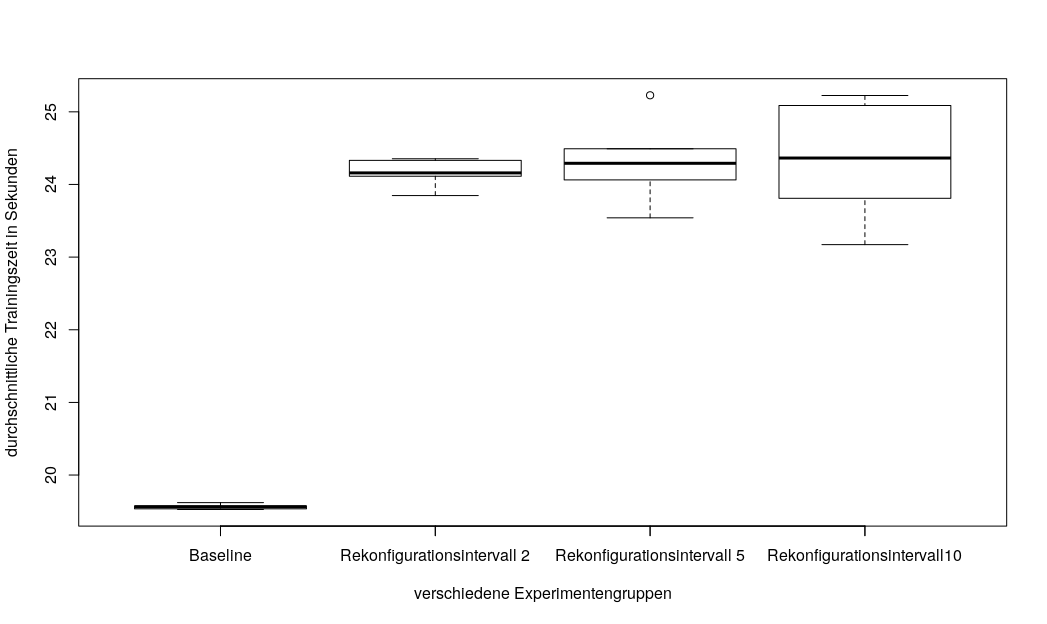
\includegraphics[width= .45\textwidth]{KapitelPartB/Images/reconf1.png}\label{abb:reconf1}}
     \hfill
     \subfloat[][]{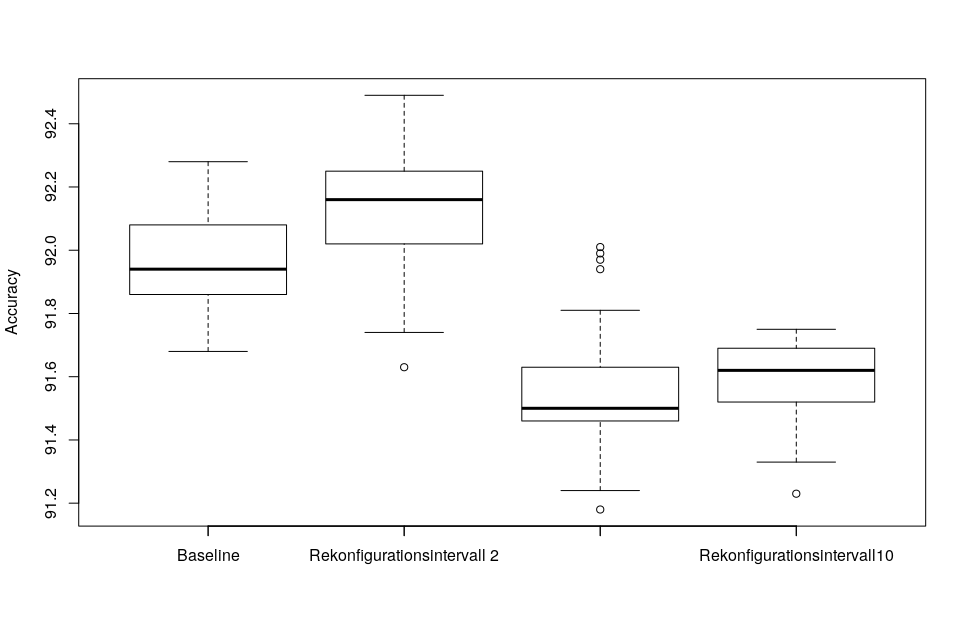
\includegraphics[width= .45\textwidth]{KapitelPartB/Images/reconf2.png}\label{abb:reconf2}}
     \\
     \subfloat[][]{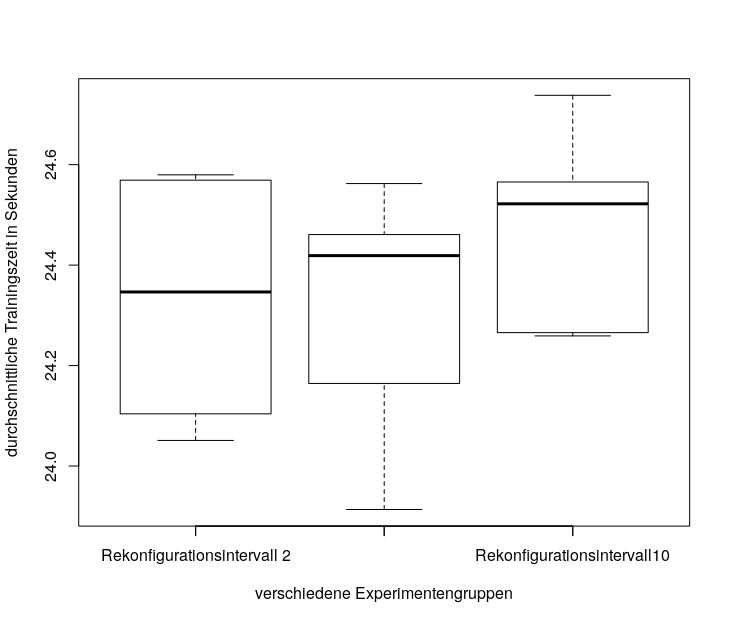
\includegraphics[width=.45\textwidth]{KapitelPartB/Images/reconf3.png}\label{abb:reconf3}}
     \caption{Experimente zum Rekonfigurationsintervall: (a) Boxplot der durchschnittlichen Trainingszeit (b) Boxplot der durchschnittlichen Trainingszeit ohne Baseline-Netz (c) Boxplot der Accuracy}
     \label{abb:reconf}
\end{figure}

In Abbildung \ref{abb:reconf3} ist zu sehen, wie sich die Accuracy bei diesen Experimenten verhält. Zu sehen ist, dass die Accuracy keine klare Tendenz hat. Dies zeigt sich auch in den t-Test in Tabelle \ref{tab:reconf2}. Hier ist die Anzahl an Experimenten wohl zu gering, um eine klare Aussage zu treffen. Da die Unterschiede hier aber so gering sind ist die Wahl des Rekonfigurationsintervall nicht so wichtig.


\begin{table}[]
\caption{p-Werte für den t-Tests zu den Accuracys der Rekonfigurationsinterval Experimente}
\begin{tabular}{l|c|c|c|c|}
\cline{2-5}
                                & \multicolumn{1}{l|}{Baseline} & \multicolumn{1}{l|}{Rekonf 2}  & \multicolumn{1}{l|}{Rekonf 5}  & \multicolumn{1}{l|}{Rekonf 10} \\ \hline
\multicolumn{1}{|l|}{Baseline}  & X                             & \cellcolor[HTML]{FFFFFF}0.0478 & \cellcolor[HTML]{FE0000}0.1111 & \cellcolor[HTML]{FFFFFF}0.0105 \\ \hline
\multicolumn{1}{|l|}{Rekonf 2}  & X                             & X                              & \cellcolor[HTML]{FE0000}0.43   & \cellcolor[HTML]{FE0000}0.1824 \\ \hline
\multicolumn{1}{|l|}{Rekonf 5}  & X                             & X                              & X                              & \cellcolor[HTML]{FE0000}0.9938 \\ \hline
\multicolumn{1}{|l|}{Rekonf 10} & X                             & X                              & X                              & X                              \\ \hline
\end{tabular}
\label{tab:reconf2}
\end{table}
 
  
\subsubsection{Experimente zur Lernrate}
Der Einfluss der Lernrate auf das Beschneiden des Netzes wird mit fünf verschiedenen Lernraten untersucht. Beginnend mit der Lernrate $0,2$ und für jede weitere der fünf Lernraten die Hälfte der vorherigen.
Die durchschnittliche Trainingszeit in Sekunden für verschiedene Lernrate ist in Abbildung \ref{abb:lr} zu sehen. Es ist deutlich zu sehen, dass mit sinkender Lernrate die Trainingszeit steigt. Das bedeutet, dass mit sinkender Lernrate weniger von Netz beschnitten wird, dies sorgt allerdings nicht zu einem verringerten Overhead. Der Overhead hängt bei diesem Verfahren von der Häufigkeit der Rekonfiguration ab.


In Tabelle \ref{tab:lr1} sind die p-Werte für die paarweisen t-Test zu sehen, die berechnen wie wahrscheinlich es ist, dass ein Fehler 1. Art auftritt. Da die p-Werte bis auf einen Wert unter dem Signifikanzniveau von $\alpha = 0,05$ ist die hier getroffene Aussage statistisch belegt.


\begin{table}[]
\caption{p-Werte für den t-Tests zu den Accuracys der durchschnittlichen Experimenten zur Lernrate}
\begin{tabular}{l|c|c|c|c|l|}
\cline{2-6}
                               & \multicolumn{1}{l|}{Baseline} & \multicolumn{1}{l|}{LR 0,2} & \multicolumn{1}{l|}{LR 0,1}                       & \multicolumn{1}{l|}{LR 0,05} & LR 0,025                       \\ \hline
\multicolumn{1}{|l|}{Baseline} & X                             & 0,0003                      & \multicolumn{1}{l|}{$5,3\cdot10^{-5}$} & \multicolumn{1}{l|}{0,0003}  & $4,9\cdot10^{-6}$   \\ \hline
\multicolumn{1}{|l|}{LR 0,2}   & X                             & X                           & 0,0001                                            & 0,0011                       & $9,2\cdot10^{-7}$   \\ \hline
\multicolumn{1}{|l|}{LR 0,1}   & X                             & X                           & X                                                 & 0,0332                       & 0.0011                         \\ \hline
\multicolumn{1}{|l|}{LR 0,05}  & X                             & X                           & X                                                 & X                            & \cellcolor[HTML]{FE0000}0,9074 \\ \hline
\multicolumn{1}{|l|}{LR 0,0250} & X                             & X                           & X                                                 & X                            & \multicolumn{1}{c|}{X}         \\ \hline
\end{tabular}
\label{tab:lr1}
\end{table}
 
 \begin{figure}
     \centering
     \subfloat[][]{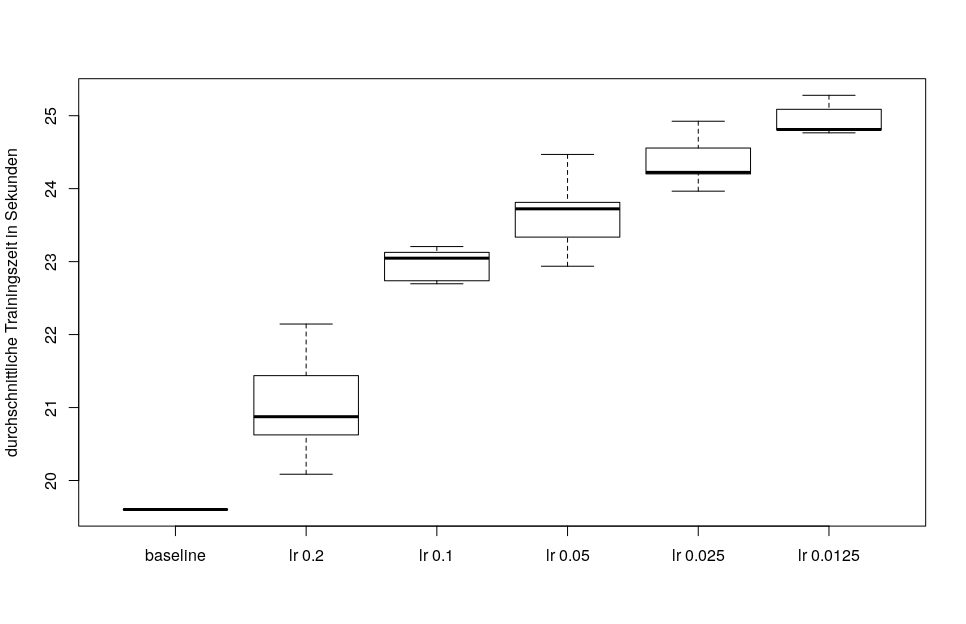
\includegraphics[width= .45\textwidth]{KapitelPartB/Images/lr1.png}\label{abb:lr1}}
     \hfill
     \subfloat[][]{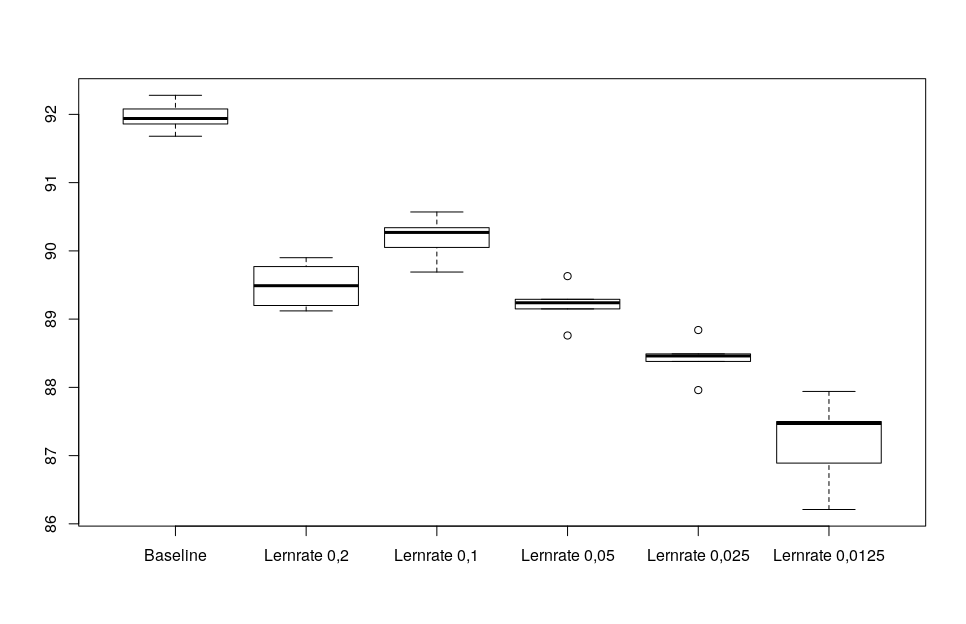
\includegraphics[width= .45\textwidth]{KapitelPartB/Images/lr2.png}\label{abb:lr2}}\\
    \subfloat[][]{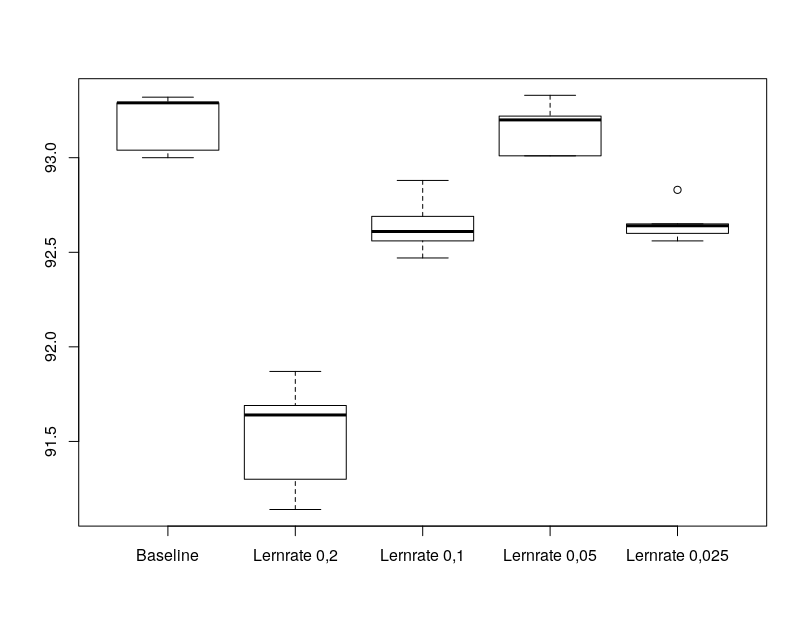
\includegraphics[width= .45\textwidth]{KapitelPartB/Images/lr3.png}\label{abb:lr3}}
     \caption{Experimente zur Lernrate: (a) Boxplot der durchschnittlichen Trainingszeit (b) Boxplot der Accuracys (c) Boxplot ausgewählter Accuracys}
     \label{abb:lr}
\end{figure}

 In Abbildung \ref{abb:lr2} sind die Accuracy der verschiedenen Lernraten abgebildet. Die Lernrate $0,05$ schneidet hier am Besten ab. Dies kann darauf zurück geführt werden, dass bei einer größeren Lernrate weniger Minima in der Verlustfunktion gefunden werden können. Der Effekt bei wesentlich kleineren Lernraten ist, dass der Trainingsprozess zwar mit jedem Schritt in die Richtung des Minimums geht, dabei aber durch die kleine Lernrate das tatsächliche Minimum innerhalb der 180 Epochen nicht erreicht wird oder mit der kleinen Lernrate ein lokales Minimum nicht verlassen werden kann. In Tabelle \ref{tab:lr2} sind die p-Werte der paarweisen t-Tests zu sehen. Bis auf zwei Werte sind diese kleiner als das Signifikanzniveau $\alpha=0,05$. Damit ist die Wahrscheinlichkeit für einen Fehler 1.Art bis auf diese zwei Werte kleiner als 5 \%. Für PruneTrain mit der Lernrate $0,05$ stellt sich die Frage ob der Effekt, dass dieser Wert hier am Besten und vergleichbar zum Baseline-Netz am Baseline-Netz selber oder an Effekten von PruneTrain liegt. Um dies zu klären wurde zusätzlich das Baseline-Netz mit der Lernrate $0,05$ trainiert. Das Ergbenis ist in Abbildung \ref{abb:lr3} zu sehen. Da das Baseline-Netz mit Lernrate $0,05$ hier wesentlich schlechter als das Baseline Netz mit Lernrate $0,1$ abschneidet ist der Effekt auf PruneTrain zurückzuführen.
 

\begin{table}[]
\caption{p-Werte für den t-Tests zu den Accuracys der Experimente zu den Lernraten}
\begin{tabular}{l|c|c|c|c|l|}
\cline{2-6}
                               & \multicolumn{1}{l|}{Baseline} & \multicolumn{1}{l|}{LR 0,2}  & \multicolumn{1}{l|}{LR 0,1} & \multicolumn{1}{l|}{LR 0,05}                        & LR 0,025                       \\ \hline
\multicolumn{1}{|l|}{Baseline} & X                             & 3,355*10\textasciicircum{}-5 & \multicolumn{1}{l|}{0,0005} & \multicolumn{1}{l|}{\cellcolor[HTML]{FE0000}0,7253} & 0,004                          \\ \hline
\multicolumn{1}{|l|}{LR 0,2}   & X                             & X                            & 0,0003                      & 4,83*10\textasciicircum{}-5                         & 0,0005                         \\ \hline
\multicolumn{1}{|l|}{LR 0,1}   & X                             & X                            & X                           & 0,0006                                              & \cellcolor[HTML]{FE0000}0,8715 \\ \hline
\multicolumn{1}{|l|}{LR 0,05}  & X                             & X                            & X                           & X                                                   & 0,0003                         \\ \hline
\multicolumn{1}{|l|}{LR 0,025} & X                             & X                            & X                           & X                                                   & \multicolumn{1}{c|}{X}         \\ \hline
\end{tabular}
\label{tab:lr2}
\end{table}
 
\subsubsection{Experimente zum Grenzwert}

Der Einfluss des gewählten Thresholds wird hier untersucht. In Abbildung \ref{abb:thres1} sind die durchschnittlichen Trainingszeiten abgebildet. Auch hier ist zu sehen, dass die durchschnittliche Trainingszeit durch die Anwendung des PruneTrain Algorithmus zunimmt.Unter einem bestimmten Threshold-Wert sind hier die durchschnittlichen Trainingszeiten nicht mehr unterscheidbar. In Tabelle \ref{tab:thres1} sind die p-Werte des t-Tests abgebildet, der untersuchen soll wo ein statistisch signifikanter Unterschied zwischen den durchschnittlichen Trainingszeiten der Experimentengruppen herrscht. Die p-Werte stützen die Aussagen.

\begin{table}[]
\caption{p-Werte für den t-Tests zu den durchschnittlichen Trainingszeiten der Experimente zum Threshold}
\begin{tabular}{l|c|c|c|c|l|}
\cline{2-6}
                                       & \multicolumn{1}{l|}{Baseline} & \multicolumn{1}{l|}{Thres. 0,1} & \multicolumn{1}{l|}{Thres. 0,01} & \multicolumn{1}{l|}{Thres. 0,001} & Thres. 0,0001               \\ \hline
\multicolumn{1}{|l|}{Baseline}         & X                             & 0.0003                             & 0.0002                              & 1.778e-05                            & 0.0002                         \\ \hline
\multicolumn{1}{|l|}{Thres. 0,1}    & X                             & X                                  & \cellcolor[HTML]{FE0000}0.0577      & 0.0018                               & 0.0479                         \\ \hline
\multicolumn{1}{|l|}{Thres. 0,01}   & X                             & X                                  & X                                   & \cellcolor[HTML]{FE0000}0.1209       & \cellcolor[HTML]{FE0000}0.9159 \\ \hline
\multicolumn{1}{|l|}{Thres. 0,001}  & X                             & X                                  & X                                   & X                                    & \cellcolor[HTML]{FE0000}0.1450 \\ \hline
\multicolumn{1}{|l|}{Thres. 0,0001} & X                             & X                                  & X                                   & X                                    & \multicolumn{1}{c|}{X}         \\ \hline
\end{tabular}
\label{tab:thres1}
\end{table}


 \begin{figure}
     \centering
     \subfloat[][]{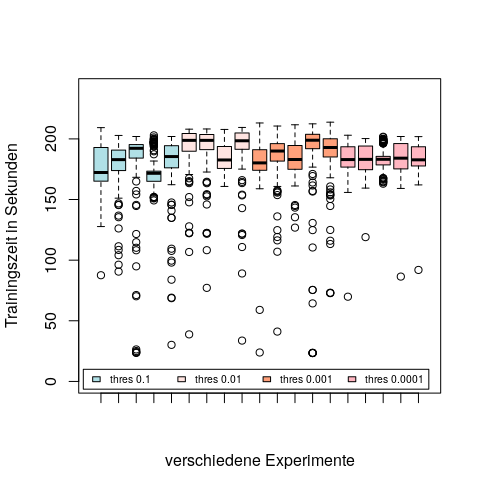
\includegraphics[width= .45\textwidth]{KapitelPartB/Images/thres1.png}\label{abb:thres1}}
     \hfill
     \subfloat[][]{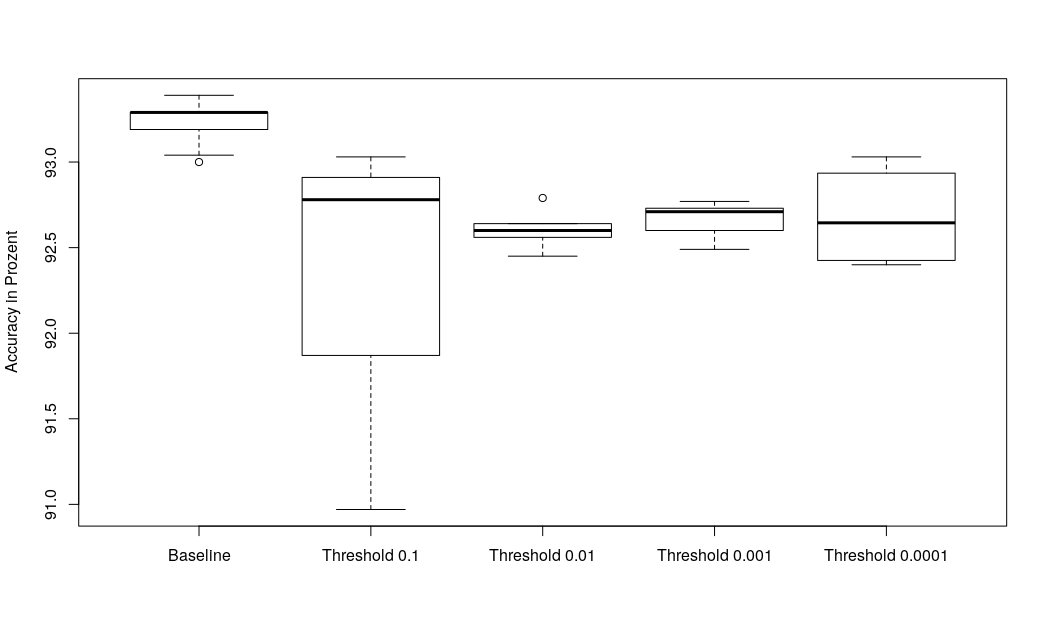
\includegraphics[width= .45\textwidth]{KapitelPartB/Images/thres2.png}\label{abb:thres2}}
     \caption{Experimente zur Threshold: (a) Boxplot der durchschnittlichen Trainingszeit (b) Boxplot der durchschnittlichen Trainingszeit ohne Baseline-Netz (c) Boxplot der Accuracys}
     \label{abb:thres}
\end{figure}
In Abbildung \ref{abb:thres2} ist die Accuracy zu sehen. Aus dieser Abbildung lässt sich keine Tendenz erkennen. Diese Aussage wird durch die p-Werte der paarweisen t-Tests in Tabelle \ref{tab:thres2} gestützt.
 \begin{table}[]
\caption{p-Werte für den t-Tests zu den Accuracys der Experimente zum Threshold}
\begin{tabular}{l|c|c|c|c|l|}
\cline{2-6}
                                     & \multicolumn{1}{l|}{Baseline} & \multicolumn{1}{l|}{Thres. 0,01} & \multicolumn{1}{l|}{Thres. 0,001} & \multicolumn{1}{l|}{Thres. 0,0001} & Thres. 0,00001                 \\ \hline
\multicolumn{1}{|l|}{Baseline}       & X                             & 0,1927                           & \multicolumn{1}{l|}{0,0002}       & \multicolumn{1}{l|}{0,0003}        & 0,0360                         \\ \hline
\multicolumn{1}{|l|}{Thres. 0,01}    & X                             & X                                & \cellcolor[HTML]{FE0000}0,6799    & \cellcolor[HTML]{FE0000}0,6121     & \cellcolor[HTML]{FE0000}0,5968 \\ \hline
\multicolumn{1}{|l|}{Thres. 0,001}   & X                             & X                                & X                                 & \cellcolor[HTML]{FE0000}0,5096     & \cellcolor[HTML]{FE0000}0,6815 \\ \hline
\multicolumn{1}{|l|}{Thres. 0,0001}  & X                             & X                                & X                                 & X                                  & \cellcolor[HTML]{FE0000}0,9076 \\ \hline
\multicolumn{1}{|l|}{Thres. 0,00001} & X                             & X                                & X                                 & X                                  & \multicolumn{1}{c|}{X}         \\ \hline
\end{tabular}
\label{tab:thres2}
\end{table}
\subsubsection{Diskussion der Methode}
Für die Evaluation des Beschneiden des Netzes werden in der Original-Veröffentlichung mehrere GPUs verwendet \cite{prunetrain}. Dies führt dazu, dass bereits in diesem Teil der Implementierung Trainingszeit durch verminderte Kommunikation zwischen den GPUs gespart wird. Da hier nur mit einer GPU evaluiert wird ergibt sich hier noch keine direkte Einsparung an Trainingszeit. Eine weitere Möglichkeit Trainingszeit zu sparen ergibt sich durch Erhöhen der Batchgröße bei kleiner werdendem Netz. Zu beachten ist hier, dass die Speicherauslastung gleich bleiben sollte und eine Vergleichbarkeit mit der Veröffentlichung zu gewährleisten. Diese Evaluierung wird in Kapitel \ref{sec:ptnew} durchgeführt.
Die Ergebnisse dieser Evaluierung lassen sich schlecht mit denen in der Originalveröffentlichung vergleichen, da dort die Wahl der Hyperparameter nicht direkt evaluiert werden.

\section{Experimente zur Anpassung der Batchgröße beim Beschneiden des Netzes}\label{sec:ptnew}

Die Anpassung der Batchgröße des Netzwerks in der Veröffentlichung arbeitet mit einer Grenze bis zu dieser der Speicher ausgelastet werden darf. 

Die Berechnung der maximalen Batchgröße für eine gegegebene Speichergrösse und Netzarchitektur wird in Kapitel \ref{sec:batch} beschrieben.

\subsection{Berechnung der Batchgröße abhängig vom Speicherverbrauch}\label{sec:batch}
Da sich in Pytorch der freie Speicher nicht direkt auslesen lässt wird mit Hilfe von Experimenten, die auf der GPU durchgeführt werden gemessen wie sich die Speicherauslastung verhält. In Abbildung \ref{abb:memory1} ist zu sehen, wie sich die Speicherauslastung proportional zur Batchgröße verhält. Es ist gut zu erkennen, dass der Zusammenhang linear ist. Die Passgenauigkeit dieses Zusammenhangs kann mittels einer linearen Regression bestimmt werden.  Daher wird mit der roten Gerade eine lineare Regression berechnet. Der maximale Abstand der gemessenen Punkte zur Gerade ist $0,19$ für Punkte, die unter der Gerade liegen sowie $0,67$ für Punkte die über der Gerade liegen. Zusammen mit der graphischen Übereinstimmung ergibt sich klar ein linearer Zusammenhang mit kleinen Abweichungen.
 \begin{figure}
     \centering
     \subfloat[][]{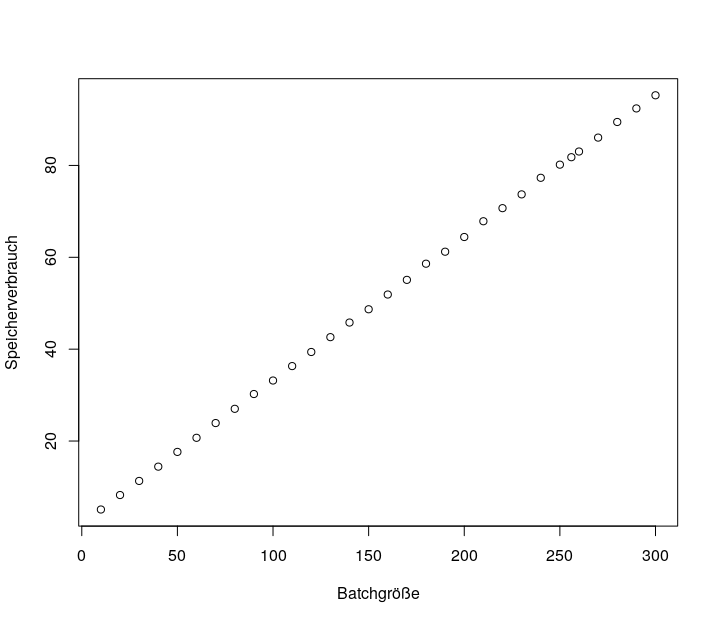
\includegraphics[width= .47\textwidth]{KapitelPartB/Images/memory1.png}\label{abb:memory1}}
     \hfill
     \subfloat[][]{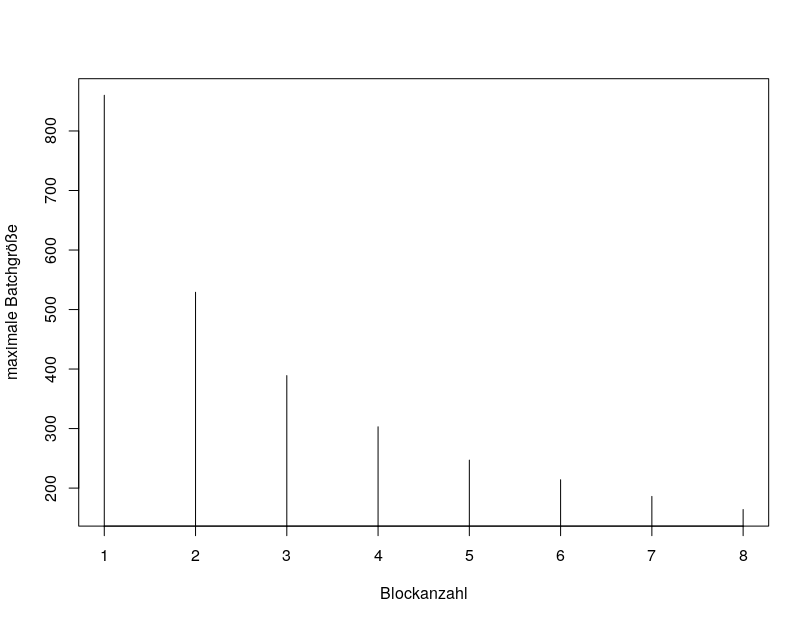
\includegraphics[width= .47\textwidth]{KapitelPartB/Images/memory2.png}\label{abb:memory2}}\\
     \subfloat[][]{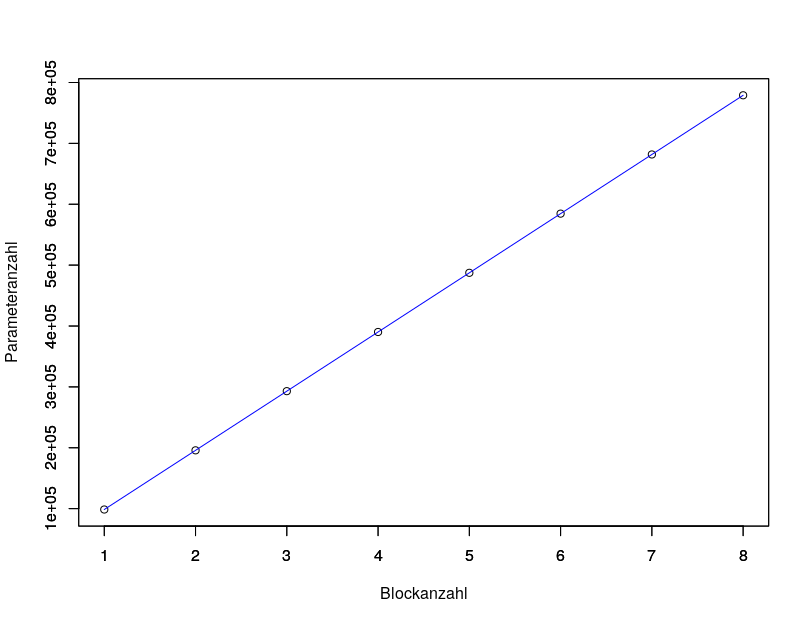
\includegraphics[width= .47\textwidth]{KapitelPartB/Images/memory3.png}\label{abb:memory3}}
     \hfill
     \subfloat[][]{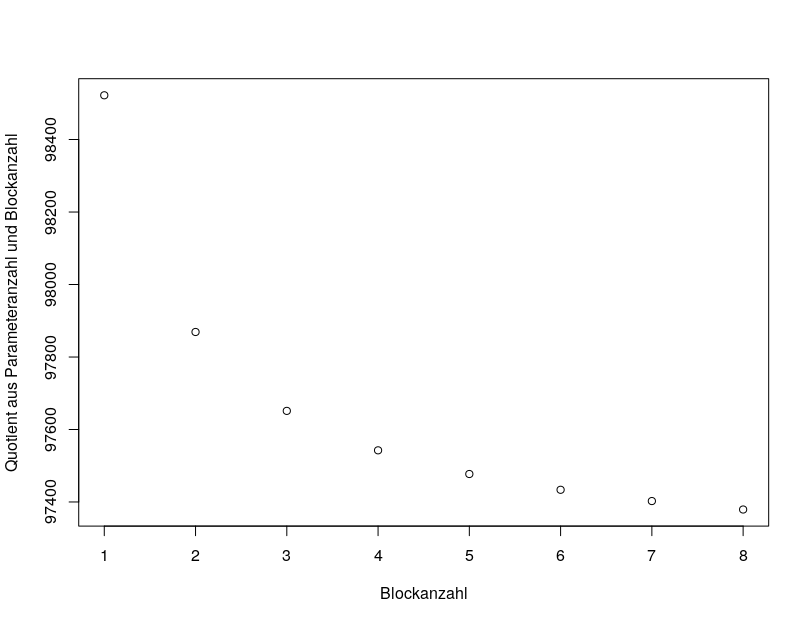
\includegraphics[width= .47\textwidth]{KapitelPartB/Images/memory4.png}\label{abb:memory4}}\\
     \subfloat[][]{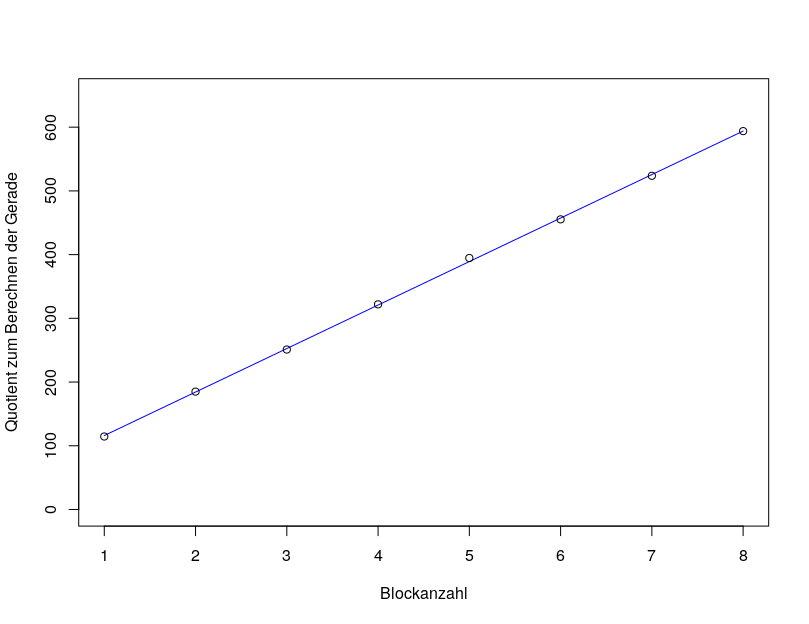
\includegraphics[width= .47\textwidth]{KapitelPartB/Images/memory5.png}\label{abb:memory5}}\\
          
     \caption{Darstellung des Berechnen der Geraden}
     \label{abb:memory}
\end{figure}
Durch diesen linearen Zusammenhang reicht es ein Modell zu bilden, welches für einen Wert des Speicherverbrauchs abhängig von der Netzarchitektur berechnet, wie groß die Batchgröße maximal sein darf. Zu diesem Zweck wird ein Netz mit drei Phasen betrachtet und ein Modell entwickelt mit dem sich die maximale Batchgröße berechnen lässt. Die maximale Batchgröße hängt ab von:

\begin{itemize}
 \item der Blockanzahl
 \item der Phasenanzahl und
 \item der Anzahl an Schichten pro Block
 \item Breite der Schichten je Phase
\end{itemize}
In Abbildung \ref{abb:memory2} ist abgebildet, wie sich die Blockanzahl bei gleichbleibender Speicherauslastung auf die maximale Batchgröße auswirkt. Die Blockanzahl wirkt sich wie zu sehen ist nicht linear auf die maximale Batchgröße aus. Die maximale Blockanzahl hängt ab von der maximalen Speicherauslastung während einer Epoche. Dies ist abhängig von der Blockgröße, da aufgrund der Kurzschlussverbindungen die Ausgabe jedes Blocks zwischengespeichert werden muss.
Betrachtet man hingegen den Zusammenhang zwischen Blockanzahl und Parameteranzahl, wie in Abbildung \ref{abb:memory3} abgebildet, so ergibt sich hier ein linearer Zusammenhang. In Abbildung \ref{abb:memory4} ist der Zusammenhang zwischen Blockanzahl und dem Quotienten aus Parameteranzahl und Blockanzahl zu sehen. Der Verlauf dieser Kurve ähnelt dem Verlauf von Abbildung \ref{abb:memory2}. In Abbildung \ref{abb:memory5} wird daher der Quotient aus diesen beiden Größen gegen die Blockanzahl abgebildet und eine Gerade mit linearer Regression berechnet.


Um die Wahrscheinlichkeit zu prüfen, dass in Abbildung \ref{abb:memory} fälschlicher Weise ein linearer Zusammenhang angenommen wird, wird ein t-Test ausgeführt.
Es ergibt sich die Alternativ- und Nullhypothese:
\begin{align*}
 H_0: \text{Es besteht kein linearer Zusammenhang zwischen dem Quotienten } G \\
 \text{und der Anzahl von Blöcken} \\
 H_1: \text{Es besteht ein linearer Zusammenhang zwischen dem Quotienten } G \\ 
 \text{ und der Anzahl von Blöcken}
\end{align*}
Mit einem Signifikanzniveau von $\alpha =0,05$ und einem $p$-Wert von $p=3,824 \cdot 10^{-12}$ ist die Nullhypothese abzulehnen, und die Alternativhypothese anzunehmen. 

Mit Hilfe dieses linearen Zusammenhangs lässt sich bei gegebener Parameteranzahl $(PA)$ und Blockanzahl $(BA)$ die maximale Batchgröße $(BG)$ berechnen:

\begin{equation}
 BG=\frac{PA}{BA\left( 68,25 \cdot BA + 47,85\right)}
\end{equation}


Da einzelne Punkte einen maximalen Abstand von $d=2,07$ zur Geraden wurde das Ergebnis durch Multiplikation mit $0,98$ ein Sicherheitsabstand eingeführt.


\subsection{Evaluierung der Anpassung der Batchgröße an die Netzgröße}

Da sich für ein gegebenes Netz die Speicherauslastung abhängig von der Batchgröße ein linearer Zusammenhang ergibt, kann die Batchgröße direkt angepasst werden, sobald das beschnittene Netz für eine Epoche trainiert hat. Es wird per Dreisatz berechnet wie groß die Batchgröße sein darf, bei gegebener maximaler Speicherauslastung. In Abbildung \ref{abb:bSize1} ist zu sehen wie sich die durchschnittliche Trainingszeit pro Epoche entwickelt, bei Anpassung der Batchgröße. Für Abbildung \ref{abb:bSize1} werden zwei verschieden große Lasso-Ratio Werte $(LaR)$ $(0,2 \text{und} 0,25)$ getestet. Bei der Lasso-Ratio von $LaR=0,25$ ergibt sich ein Gewinn an durchschnittlicher Trainingszeit pro Epoche. Zum Vergleich enthält die Abbildung auch die entsprechenden Experimente aus den Experimente zur Lasso-Ratio ohne Anpassung der Batchgröße. Die durchschnittliche Trainingszeit sinkt signifikant im Vergleich zum entsprechenden Experiment ohne Anpassung der Batchgröße, da mit einer höheren Batchgröße weniger Durchläufe gebraucht werden um die Epoche abzuschliessen. Für die Lasso-Ratio von $LaR=0,25$ ergibt sich bei einem t-Test ein p-Wert von $p=6.445\cdot 10^{-05}$. Für die Lasso-Ratio von $LaR=0,2$ ergibt sich bei einem t-Test ein p-Wert von $p=0,0004$. 



 \begin{figure}
     \centering
     \subfloat[][]{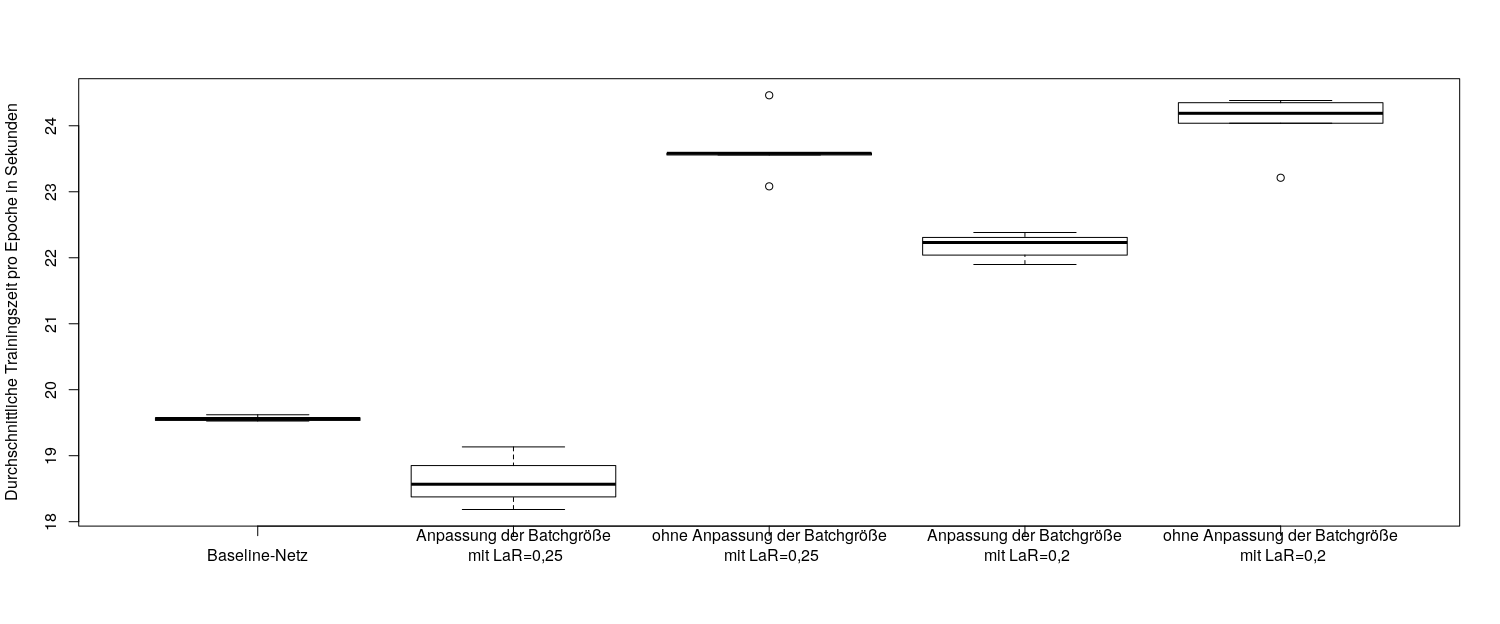
\includegraphics[width= .75\textwidth]{KapitelPartB/Images/bSize1.png}\label{abb:bSize1}}
     \hfill
     \subfloat[][]{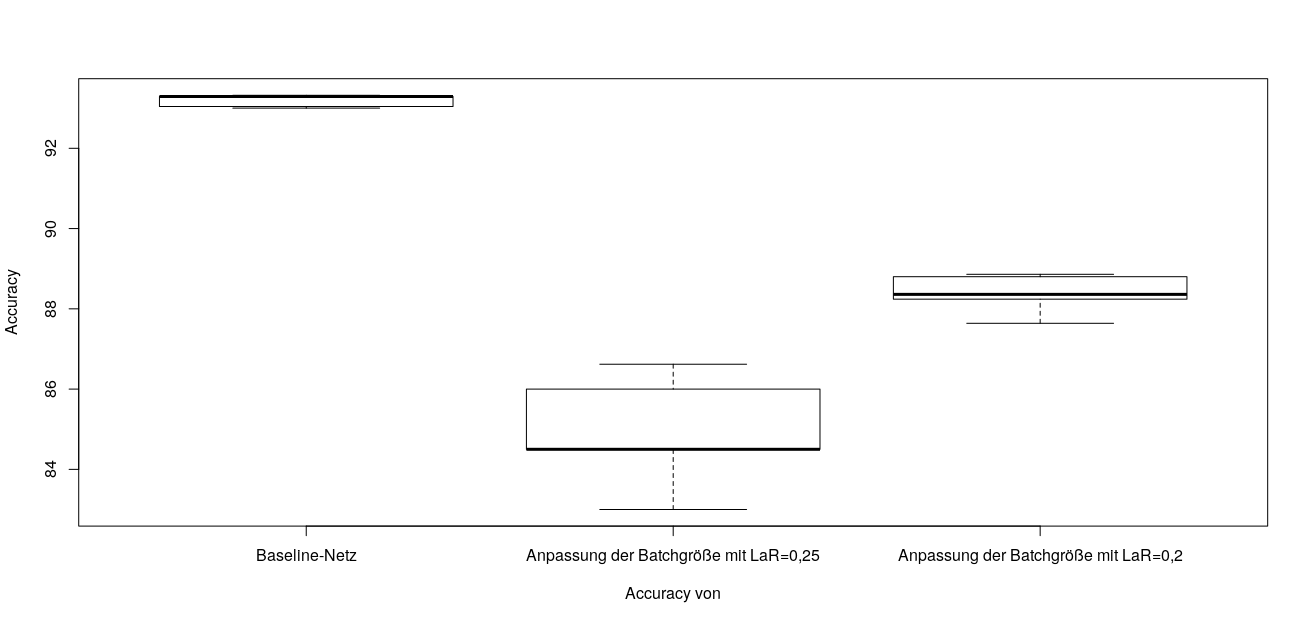
\includegraphics[width= .75\textwidth]{KapitelPartB/Images/bSize2.png}\label{abb:bSize2}}\\
     \caption{Vergleich von (a) Durchschnittlicher Trainingszeit (b) Accuracys von PruneTrain mit Anpassung der Batchgrößeund Baseline-Netz}
     \label{abb:bSize}
\end{figure}

In Abbildung \ref{abb:bSize2} ist zu sehen, wie gross der Accuracy-Verlust für das PruneTrain-Netz mit Anpassung der Batchgröße ist. Für PruneTrain mit einer Lasso-Ratio von 0,2 ergibt sich ein Accuracy Verlust von durchschnittlich 4,18 \%. Für eine höhere Lasso-Ratio ergibt sich ein Accuracy-Verlust von 7,24 \%. Diese Verluste sind wahrscheinlich auf eine nicht passende Anpassung der Lernrate in Abhängigkeit von der Änderung der Batchgröße zurückzuführen oder einer weniger häufigen Anpassung der Gewichte. Lernrate und Batchgröße hängen durch die ANzahl an Anpassungen der Gewichte zusammen: Steigt die Batchgröße, so werden weniger Durchläufe und damit weniger Gewichtsanpassungen durchgeführt. Um den geringeren zurück gelegten Weg in Richtung eines Minimum zu kopmensieren kann die Lernrate erhöht werden.











